% Created by tikzDevice version 0.12.3 on 2020-06-01 10:21:30
% !TEX encoding = UTF-8 Unicode
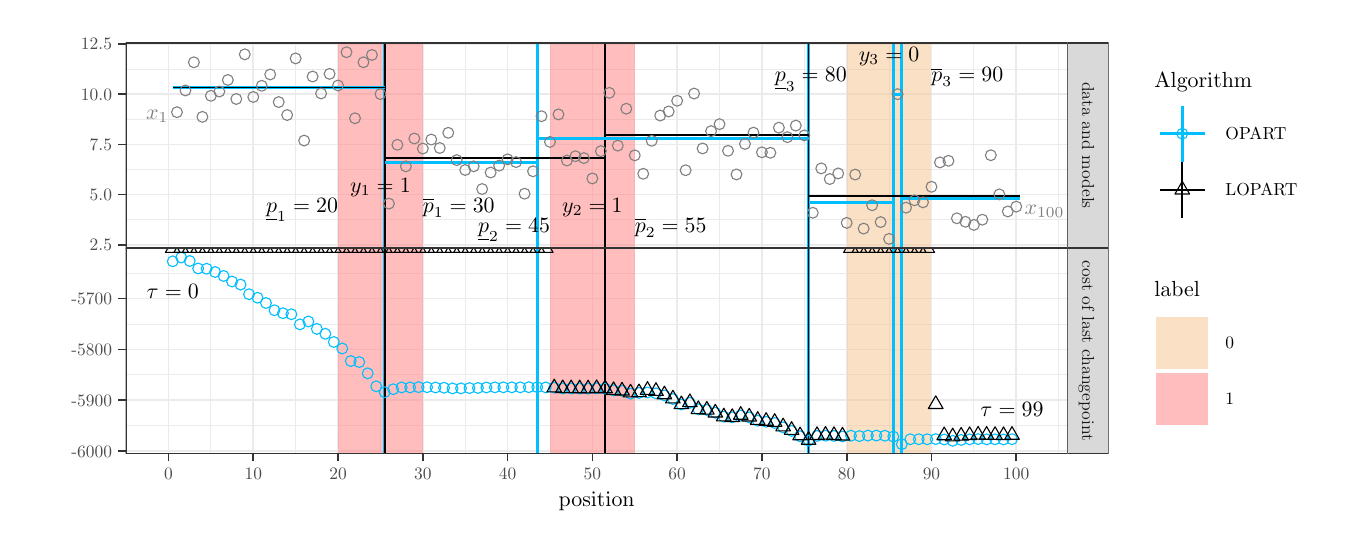
\begin{tikzpicture}[x=1pt,y=1pt]
\definecolor{fillColor}{RGB}{255,255,255}
\path[use as bounding box,fill=fillColor,fill opacity=0.00] (0,0) rectangle (469.75,180.67);
\begin{scope}
\path[clip] (  0.00,  0.00) rectangle (469.75,180.67);
\definecolor{drawColor}{RGB}{255,255,255}
\definecolor{fillColor}{RGB}{255,255,255}

\path[draw=drawColor,line width= 0.6pt,line join=round,line cap=round,fill=fillColor] (  0.00,  0.00) rectangle (469.76,180.68);
\end{scope}
\begin{scope}
\path[clip] ( 35.41,100.98) rectangle (375.76,175.17);
\definecolor{fillColor}{RGB}{255,255,255}

\path[fill=fillColor] ( 35.41,100.98) rectangle (375.76,175.18);
\definecolor{drawColor}{gray}{0.92}

\path[draw=drawColor,line width= 0.3pt,line join=round] ( 35.41,111.30) --
	(375.76,111.30);

\path[draw=drawColor,line width= 0.3pt,line join=round] ( 35.41,129.44) --
	(375.76,129.44);

\path[draw=drawColor,line width= 0.3pt,line join=round] ( 35.41,147.57) --
	(375.76,147.57);

\path[draw=drawColor,line width= 0.3pt,line join=round] ( 35.41,165.70) --
	(375.76,165.70);

\path[draw=drawColor,line width= 0.3pt,line join=round] ( 35.57,100.98) --
	( 35.57,175.17);

\path[draw=drawColor,line width= 0.3pt,line join=round] ( 66.20,100.98) --
	( 66.20,175.17);

\path[draw=drawColor,line width= 0.3pt,line join=round] ( 96.83,100.98) --
	( 96.83,175.17);

\path[draw=drawColor,line width= 0.3pt,line join=round] (127.47,100.98) --
	(127.47,175.17);

\path[draw=drawColor,line width= 0.3pt,line join=round] (158.10,100.98) --
	(158.10,175.17);

\path[draw=drawColor,line width= 0.3pt,line join=round] (188.74,100.98) --
	(188.74,175.17);

\path[draw=drawColor,line width= 0.3pt,line join=round] (219.37,100.98) --
	(219.37,175.17);

\path[draw=drawColor,line width= 0.3pt,line join=round] (250.00,100.98) --
	(250.00,175.17);

\path[draw=drawColor,line width= 0.3pt,line join=round] (280.64,100.98) --
	(280.64,175.17);

\path[draw=drawColor,line width= 0.3pt,line join=round] (311.27,100.98) --
	(311.27,175.17);

\path[draw=drawColor,line width= 0.3pt,line join=round] (341.91,100.98) --
	(341.91,175.17);

\path[draw=drawColor,line width= 0.3pt,line join=round] (372.54,100.98) --
	(372.54,175.17);

\path[draw=drawColor,line width= 0.6pt,line join=round] ( 35.41,102.24) --
	(375.76,102.24);

\path[draw=drawColor,line width= 0.6pt,line join=round] ( 35.41,120.37) --
	(375.76,120.37);

\path[draw=drawColor,line width= 0.6pt,line join=round] ( 35.41,138.50) --
	(375.76,138.50);

\path[draw=drawColor,line width= 0.6pt,line join=round] ( 35.41,156.64) --
	(375.76,156.64);

\path[draw=drawColor,line width= 0.6pt,line join=round] ( 35.41,174.77) --
	(375.76,174.77);

\path[draw=drawColor,line width= 0.6pt,line join=round] ( 50.88,100.98) --
	( 50.88,175.17);

\path[draw=drawColor,line width= 0.6pt,line join=round] ( 81.52,100.98) --
	( 81.52,175.17);

\path[draw=drawColor,line width= 0.6pt,line join=round] (112.15,100.98) --
	(112.15,175.17);

\path[draw=drawColor,line width= 0.6pt,line join=round] (142.79,100.98) --
	(142.79,175.17);

\path[draw=drawColor,line width= 0.6pt,line join=round] (173.42,100.98) --
	(173.42,175.17);

\path[draw=drawColor,line width= 0.6pt,line join=round] (204.05,100.98) --
	(204.05,175.17);

\path[draw=drawColor,line width= 0.6pt,line join=round] (234.69,100.98) --
	(234.69,175.17);

\path[draw=drawColor,line width= 0.6pt,line join=round] (265.32,100.98) --
	(265.32,175.17);

\path[draw=drawColor,line width= 0.6pt,line join=round] (295.95,100.98) --
	(295.95,175.17);

\path[draw=drawColor,line width= 0.6pt,line join=round] (326.59,100.98) --
	(326.59,175.17);

\path[draw=drawColor,line width= 0.6pt,line join=round] (357.22,100.98) --
	(357.22,175.17);
\definecolor{drawColor}{gray}{0.50}

\node[text=drawColor,anchor=base east,inner sep=0pt, outer sep=0pt, scale=  0.79] at ( 50.88,147.42) {$x_{1}$};

\node[text=drawColor,anchor=base west,inner sep=0pt, outer sep=0pt, scale=  0.79] at (360.29,113.29) {$x_{100}$};
\definecolor{fillColor}{RGB}{255,125,125}

\path[fill=fillColor,fill opacity=0.50] (112.15,100.98) rectangle (142.79,175.17);

\path[fill=fillColor,fill opacity=0.50] (188.74,100.98) rectangle (219.37,175.17);
\definecolor{fillColor}{RGB}{246,196,143}

\path[fill=fillColor,fill opacity=0.50] (295.95,100.98) rectangle (326.59,175.17);
\definecolor{drawColor}{RGB}{0,191,255}

\path[draw=drawColor,line width= 1.1pt,line join=round] (129.00,100.98) -- (129.00,175.17);

\path[draw=drawColor,line width= 1.1pt,line join=round] (184.14,100.98) -- (184.14,175.17);

\path[draw=drawColor,line width= 1.1pt,line join=round] (282.17,100.98) -- (282.17,175.17);

\path[draw=drawColor,line width= 1.1pt,line join=round] (312.80,100.98) -- (312.80,175.17);

\path[draw=drawColor,line width= 1.1pt,line join=round] (315.87,100.98) -- (315.87,175.17);
\definecolor{drawColor}{RGB}{0,0,0}

\path[draw=drawColor,line width= 0.6pt,line join=round] (129.00,100.98) -- (129.00,175.17);

\path[draw=drawColor,line width= 0.6pt,line join=round] (208.65,100.98) -- (208.65,175.17);

\path[draw=drawColor,line width= 0.6pt,line join=round] (282.17,100.98) -- (282.17,175.17);
\definecolor{drawColor}{RGB}{0,191,255}

\path[draw=drawColor,line width= 1.1pt,line join=round] ( 52.42,159.06) -- (129.00,159.06);

\path[draw=drawColor,line width= 1.1pt,line join=round] (129.00,131.80) -- (184.14,131.80);

\path[draw=drawColor,line width= 1.1pt,line join=round] (184.14,140.73) -- (282.17,140.73);

\path[draw=drawColor,line width= 1.1pt,line join=round] (282.17,117.47) -- (312.80,117.47);

\path[draw=drawColor,line width= 1.1pt,line join=round] (312.80,156.64) -- (315.87,156.64);

\path[draw=drawColor,line width= 1.1pt,line join=round] (315.87,119.10) -- (358.75,119.10);
\definecolor{drawColor}{RGB}{0,0,0}

\path[draw=drawColor,line width= 0.6pt,line join=round] ( 52.42,159.06) -- (129.00,159.06);

\path[draw=drawColor,line width= 0.6pt,line join=round] (129.00,133.56) -- (208.65,133.56);

\path[draw=drawColor,line width= 0.6pt,line join=round] (208.65,141.81) -- (282.17,141.81);

\path[draw=drawColor,line width= 0.6pt,line join=round] (282.17,119.95) -- (358.75,119.95);
\definecolor{drawColor}{gray}{0.50}

\path[draw=drawColor,line width= 0.4pt,line join=round,line cap=round] ( 53.95,150.13) circle (  1.96);

\path[draw=drawColor,line width= 0.4pt,line join=round,line cap=round] ( 57.01,157.98) circle (  1.96);

\path[draw=drawColor,line width= 0.4pt,line join=round,line cap=round] ( 60.07,168.15) circle (  1.96);

\path[draw=drawColor,line width= 0.4pt,line join=round,line cap=round] ( 63.14,148.44) circle (  1.96);

\path[draw=drawColor,line width= 0.4pt,line join=round,line cap=round] ( 66.20,156.05) circle (  1.96);

\path[draw=drawColor,line width= 0.4pt,line join=round,line cap=round] ( 69.26,157.60) circle (  1.96);

\path[draw=drawColor,line width= 0.4pt,line join=round,line cap=round] ( 72.33,161.77) circle (  1.96);

\path[draw=drawColor,line width= 0.4pt,line join=round,line cap=round] ( 75.39,154.90) circle (  1.96);

\path[draw=drawColor,line width= 0.4pt,line join=round,line cap=round] ( 78.45,171.03) circle (  1.96);

\path[draw=drawColor,line width= 0.4pt,line join=round,line cap=round] ( 81.52,155.63) circle (  1.96);

\path[draw=drawColor,line width= 0.4pt,line join=round,line cap=round] ( 84.58,159.67) circle (  1.96);

\path[draw=drawColor,line width= 0.4pt,line join=round,line cap=round] ( 87.64,163.76) circle (  1.96);

\path[draw=drawColor,line width= 0.4pt,line join=round,line cap=round] ( 90.71,153.79) circle (  1.96);

\path[draw=drawColor,line width= 0.4pt,line join=round,line cap=round] ( 93.77,149.10) circle (  1.96);

\path[draw=drawColor,line width= 0.4pt,line join=round,line cap=round] ( 96.83,169.56) circle (  1.96);

\path[draw=drawColor,line width= 0.4pt,line join=round,line cap=round] ( 99.90,139.87) circle (  1.96);

\path[draw=drawColor,line width= 0.4pt,line join=round,line cap=round] (102.96,163.01) circle (  1.96);

\path[draw=drawColor,line width= 0.4pt,line join=round,line cap=round] (106.02,156.90) circle (  1.96);

\path[draw=drawColor,line width= 0.4pt,line join=round,line cap=round] (109.09,163.98) circle (  1.96);

\path[draw=drawColor,line width= 0.4pt,line join=round,line cap=round] (112.15,159.77) circle (  1.96);

\path[draw=drawColor,line width= 0.4pt,line join=round,line cap=round] (115.21,171.80) circle (  1.96);

\path[draw=drawColor,line width= 0.4pt,line join=round,line cap=round] (118.28,147.93) circle (  1.96);

\path[draw=drawColor,line width= 0.4pt,line join=round,line cap=round] (121.34,168.17) circle (  1.96);

\path[draw=drawColor,line width= 0.4pt,line join=round,line cap=round] (124.40,170.81) circle (  1.96);

\path[draw=drawColor,line width= 0.4pt,line join=round,line cap=round] (127.47,156.67) circle (  1.96);

\path[draw=drawColor,line width= 0.4pt,line join=round,line cap=round] (130.53,117.09) circle (  1.96);

\path[draw=drawColor,line width= 0.4pt,line join=round,line cap=round] (133.60,138.34) circle (  1.96);

\path[draw=drawColor,line width= 0.4pt,line join=round,line cap=round] (136.66,130.55) circle (  1.96);

\path[draw=drawColor,line width= 0.4pt,line join=round,line cap=round] (139.72,140.62) circle (  1.96);

\path[draw=drawColor,line width= 0.4pt,line join=round,line cap=round] (142.79,136.98) circle (  1.96);

\path[draw=drawColor,line width= 0.4pt,line join=round,line cap=round] (145.85,140.24) circle (  1.96);

\path[draw=drawColor,line width= 0.4pt,line join=round,line cap=round] (148.91,137.19) circle (  1.96);

\path[draw=drawColor,line width= 0.4pt,line join=round,line cap=round] (151.98,142.68) circle (  1.96);

\path[draw=drawColor,line width= 0.4pt,line join=round,line cap=round] (155.04,132.82) circle (  1.96);

\path[draw=drawColor,line width= 0.4pt,line join=round,line cap=round] (158.10,129.24) circle (  1.96);

\path[draw=drawColor,line width= 0.4pt,line join=round,line cap=round] (161.17,130.56) circle (  1.96);

\path[draw=drawColor,line width= 0.4pt,line join=round,line cap=round] (164.23,122.36) circle (  1.96);

\path[draw=drawColor,line width= 0.4pt,line join=round,line cap=round] (167.29,128.33) circle (  1.96);

\path[draw=drawColor,line width= 0.4pt,line join=round,line cap=round] (170.36,130.82) circle (  1.96);

\path[draw=drawColor,line width= 0.4pt,line join=round,line cap=round] (173.42,133.09) circle (  1.96);

\path[draw=drawColor,line width= 0.4pt,line join=round,line cap=round] (176.48,132.09) circle (  1.96);

\path[draw=drawColor,line width= 0.4pt,line join=round,line cap=round] (179.55,120.67) circle (  1.96);

\path[draw=drawColor,line width= 0.4pt,line join=round,line cap=round] (182.61,128.77) circle (  1.96);

\path[draw=drawColor,line width= 0.4pt,line join=round,line cap=round] (185.67,148.68) circle (  1.96);

\path[draw=drawColor,line width= 0.4pt,line join=round,line cap=round] (188.74,139.39) circle (  1.96);

\path[draw=drawColor,line width= 0.4pt,line join=round,line cap=round] (191.80,149.32) circle (  1.96);

\path[draw=drawColor,line width= 0.4pt,line join=round,line cap=round] (194.86,132.66) circle (  1.96);

\path[draw=drawColor,line width= 0.4pt,line join=round,line cap=round] (197.93,134.22) circle (  1.96);

\path[draw=drawColor,line width= 0.4pt,line join=round,line cap=round] (200.99,133.54) circle (  1.96);

\path[draw=drawColor,line width= 0.4pt,line join=round,line cap=round] (204.05,126.18) circle (  1.96);

\path[draw=drawColor,line width= 0.4pt,line join=round,line cap=round] (207.12,136.05) circle (  1.96);

\path[draw=drawColor,line width= 0.4pt,line join=round,line cap=round] (210.18,157.12) circle (  1.96);

\path[draw=drawColor,line width= 0.4pt,line join=round,line cap=round] (213.24,138.05) circle (  1.96);

\path[draw=drawColor,line width= 0.4pt,line join=round,line cap=round] (216.31,151.38) circle (  1.96);

\path[draw=drawColor,line width= 0.4pt,line join=round,line cap=round] (219.37,134.53) circle (  1.96);

\path[draw=drawColor,line width= 0.4pt,line join=round,line cap=round] (222.43,127.87) circle (  1.96);

\path[draw=drawColor,line width= 0.4pt,line join=round,line cap=round] (225.50,139.79) circle (  1.96);

\path[draw=drawColor,line width= 0.4pt,line join=round,line cap=round] (228.56,148.92) circle (  1.96);

\path[draw=drawColor,line width= 0.4pt,line join=round,line cap=round] (231.62,150.39) circle (  1.96);

\path[draw=drawColor,line width= 0.4pt,line join=round,line cap=round] (234.69,154.26) circle (  1.96);

\path[draw=drawColor,line width= 0.4pt,line join=round,line cap=round] (237.75,129.16) circle (  1.96);

\path[draw=drawColor,line width= 0.4pt,line join=round,line cap=round] (240.81,156.86) circle (  1.96);

\path[draw=drawColor,line width= 0.4pt,line join=round,line cap=round] (243.88,137.03) circle (  1.96);

\path[draw=drawColor,line width= 0.4pt,line join=round,line cap=round] (246.94,143.28) circle (  1.96);

\path[draw=drawColor,line width= 0.4pt,line join=round,line cap=round] (250.00,145.80) circle (  1.96);

\path[draw=drawColor,line width= 0.4pt,line join=round,line cap=round] (253.07,136.18) circle (  1.96);

\path[draw=drawColor,line width= 0.4pt,line join=round,line cap=round] (256.13,127.63) circle (  1.96);

\path[draw=drawColor,line width= 0.4pt,line join=round,line cap=round] (259.19,138.65) circle (  1.96);

\path[draw=drawColor,line width= 0.4pt,line join=round,line cap=round] (262.26,142.74) circle (  1.96);

\path[draw=drawColor,line width= 0.4pt,line join=round,line cap=round] (265.32,135.63) circle (  1.96);

\path[draw=drawColor,line width= 0.4pt,line join=round,line cap=round] (268.38,135.45) circle (  1.96);

\path[draw=drawColor,line width= 0.4pt,line join=round,line cap=round] (271.45,144.53) circle (  1.96);

\path[draw=drawColor,line width= 0.4pt,line join=round,line cap=round] (274.51,141.10) circle (  1.96);

\path[draw=drawColor,line width= 0.4pt,line join=round,line cap=round] (277.57,145.28) circle (  1.96);

\path[draw=drawColor,line width= 0.4pt,line join=round,line cap=round] (280.64,141.74) circle (  1.96);

\path[draw=drawColor,line width= 0.4pt,line join=round,line cap=round] (283.70,113.79) circle (  1.96);

\path[draw=drawColor,line width= 0.4pt,line join=round,line cap=round] (286.76,129.82) circle (  1.96);

\path[draw=drawColor,line width= 0.4pt,line join=round,line cap=round] (289.83,125.97) circle (  1.96);

\path[draw=drawColor,line width= 0.4pt,line join=round,line cap=round] (292.89,128.00) circle (  1.96);

\path[draw=drawColor,line width= 0.4pt,line join=round,line cap=round] (295.95,110.14) circle (  1.96);

\path[draw=drawColor,line width= 0.4pt,line join=round,line cap=round] (299.02,127.59) circle (  1.96);

\path[draw=drawColor,line width= 0.4pt,line join=round,line cap=round] (302.08,108.07) circle (  1.96);

\path[draw=drawColor,line width= 0.4pt,line join=round,line cap=round] (305.14,116.50) circle (  1.96);

\path[draw=drawColor,line width= 0.4pt,line join=round,line cap=round] (308.21,110.42) circle (  1.96);

\path[draw=drawColor,line width= 0.4pt,line join=round,line cap=round] (311.27,104.35) circle (  1.96);

\path[draw=drawColor,line width= 0.4pt,line join=round,line cap=round] (314.34,156.64) circle (  1.96);

\path[draw=drawColor,line width= 0.4pt,line join=round,line cap=round] (317.40,115.63) circle (  1.96);

\path[draw=drawColor,line width= 0.4pt,line join=round,line cap=round] (320.46,118.30) circle (  1.96);

\path[draw=drawColor,line width= 0.4pt,line join=round,line cap=round] (323.53,117.56) circle (  1.96);

\path[draw=drawColor,line width= 0.4pt,line join=round,line cap=round] (326.59,123.17) circle (  1.96);

\path[draw=drawColor,line width= 0.4pt,line join=round,line cap=round] (329.65,131.98) circle (  1.96);

\path[draw=drawColor,line width= 0.4pt,line join=round,line cap=round] (332.72,132.56) circle (  1.96);

\path[draw=drawColor,line width= 0.4pt,line join=round,line cap=round] (335.78,111.78) circle (  1.96);

\path[draw=drawColor,line width= 0.4pt,line join=round,line cap=round] (338.84,110.52) circle (  1.96);

\path[draw=drawColor,line width= 0.4pt,line join=round,line cap=round] (341.91,109.40) circle (  1.96);

\path[draw=drawColor,line width= 0.4pt,line join=round,line cap=round] (344.97,111.28) circle (  1.96);

\path[draw=drawColor,line width= 0.4pt,line join=round,line cap=round] (348.03,134.58) circle (  1.96);

\path[draw=drawColor,line width= 0.4pt,line join=round,line cap=round] (351.10,120.43) circle (  1.96);

\path[draw=drawColor,line width= 0.4pt,line join=round,line cap=round] (354.16,114.26) circle (  1.96);

\path[draw=drawColor,line width= 0.4pt,line join=round,line cap=round] (357.22,116.01) circle (  1.96);
\definecolor{drawColor}{RGB}{0,0,0}

\node[text=drawColor,anchor=base east,inner sep=0pt, outer sep=0pt, scale=  0.79] at (112.15,114.03) {$\underline p_{1}=20$};

\node[text=drawColor,anchor=base east,inner sep=0pt, outer sep=0pt, scale=  0.79] at (188.74,106.77) {$\underline p_{2}=45$};

\node[text=drawColor,anchor=base east,inner sep=0pt, outer sep=0pt, scale=  0.79] at (295.95,161.18) {$\underline p_{3}=80$};

\node[text=drawColor,anchor=base,inner sep=0pt, outer sep=0pt, scale=  0.79] at (127.47,121.28) {$y_{1}=1$};

\node[text=drawColor,anchor=base,inner sep=0pt, outer sep=0pt, scale=  0.79] at (204.05,114.03) {$y_{2}=1$};

\node[text=drawColor,anchor=base,inner sep=0pt, outer sep=0pt, scale=  0.79] at (311.27,168.43) {$y_{3}=0$};

\node[text=drawColor,anchor=base west,inner sep=0pt, outer sep=0pt, scale=  0.79] at (142.79,114.03) {$\overline p_{1}=30$};

\node[text=drawColor,anchor=base west,inner sep=0pt, outer sep=0pt, scale=  0.79] at (219.37,106.77) {$\overline p_{2}=55$};

\node[text=drawColor,anchor=base west,inner sep=0pt, outer sep=0pt, scale=  0.79] at (326.59,161.18) {$\overline p_{3}=90$};
\definecolor{drawColor}{gray}{0.20}

\path[draw=drawColor,line width= 0.6pt,line join=round,line cap=round] ( 35.41,100.98) rectangle (375.76,175.18);
\end{scope}
\begin{scope}
\path[clip] ( 35.41, 26.79) rectangle (375.76,100.98);
\definecolor{fillColor}{RGB}{255,255,255}

\path[fill=fillColor] ( 35.41, 26.79) rectangle (375.76,100.98);
\definecolor{drawColor}{gray}{0.92}

\path[draw=drawColor,line width= 0.3pt,line join=round] ( 35.41, 36.83) --
	(375.76, 36.83);

\path[draw=drawColor,line width= 0.3pt,line join=round] ( 35.41, 55.20) --
	(375.76, 55.20);

\path[draw=drawColor,line width= 0.3pt,line join=round] ( 35.41, 73.58) --
	(375.76, 73.58);

\path[draw=drawColor,line width= 0.3pt,line join=round] ( 35.41, 91.95) --
	(375.76, 91.95);

\path[draw=drawColor,line width= 0.3pt,line join=round] ( 35.57, 26.79) --
	( 35.57,100.98);

\path[draw=drawColor,line width= 0.3pt,line join=round] ( 66.20, 26.79) --
	( 66.20,100.98);

\path[draw=drawColor,line width= 0.3pt,line join=round] ( 96.83, 26.79) --
	( 96.83,100.98);

\path[draw=drawColor,line width= 0.3pt,line join=round] (127.47, 26.79) --
	(127.47,100.98);

\path[draw=drawColor,line width= 0.3pt,line join=round] (158.10, 26.79) --
	(158.10,100.98);

\path[draw=drawColor,line width= 0.3pt,line join=round] (188.74, 26.79) --
	(188.74,100.98);

\path[draw=drawColor,line width= 0.3pt,line join=round] (219.37, 26.79) --
	(219.37,100.98);

\path[draw=drawColor,line width= 0.3pt,line join=round] (250.00, 26.79) --
	(250.00,100.98);

\path[draw=drawColor,line width= 0.3pt,line join=round] (280.64, 26.79) --
	(280.64,100.98);

\path[draw=drawColor,line width= 0.3pt,line join=round] (311.27, 26.79) --
	(311.27,100.98);

\path[draw=drawColor,line width= 0.3pt,line join=round] (341.91, 26.79) --
	(341.91,100.98);

\path[draw=drawColor,line width= 0.3pt,line join=round] (372.54, 26.79) --
	(372.54,100.98);

\path[draw=drawColor,line width= 0.6pt,line join=round] ( 35.41, 27.64) --
	(375.76, 27.64);

\path[draw=drawColor,line width= 0.6pt,line join=round] ( 35.41, 46.02) --
	(375.76, 46.02);

\path[draw=drawColor,line width= 0.6pt,line join=round] ( 35.41, 64.39) --
	(375.76, 64.39);

\path[draw=drawColor,line width= 0.6pt,line join=round] ( 35.41, 82.77) --
	(375.76, 82.77);

\path[draw=drawColor,line width= 0.6pt,line join=round] ( 50.88, 26.79) --
	( 50.88,100.98);

\path[draw=drawColor,line width= 0.6pt,line join=round] ( 81.52, 26.79) --
	( 81.52,100.98);

\path[draw=drawColor,line width= 0.6pt,line join=round] (112.15, 26.79) --
	(112.15,100.98);

\path[draw=drawColor,line width= 0.6pt,line join=round] (142.79, 26.79) --
	(142.79,100.98);

\path[draw=drawColor,line width= 0.6pt,line join=round] (173.42, 26.79) --
	(173.42,100.98);

\path[draw=drawColor,line width= 0.6pt,line join=round] (204.05, 26.79) --
	(204.05,100.98);

\path[draw=drawColor,line width= 0.6pt,line join=round] (234.69, 26.79) --
	(234.69,100.98);

\path[draw=drawColor,line width= 0.6pt,line join=round] (265.32, 26.79) --
	(265.32,100.98);

\path[draw=drawColor,line width= 0.6pt,line join=round] (295.95, 26.79) --
	(295.95,100.98);

\path[draw=drawColor,line width= 0.6pt,line join=round] (326.59, 26.79) --
	(326.59,100.98);

\path[draw=drawColor,line width= 0.6pt,line join=round] (357.22, 26.79) --
	(357.22,100.98);
\definecolor{fillColor}{RGB}{255,125,125}

\path[fill=fillColor,fill opacity=0.50] (112.15, 26.79) rectangle (142.79,100.98);

\path[fill=fillColor,fill opacity=0.50] (188.74, 26.79) rectangle (219.37,100.98);
\definecolor{fillColor}{RGB}{246,196,143}

\path[fill=fillColor,fill opacity=0.50] (295.95, 26.79) rectangle (326.59,100.98);
\definecolor{drawColor}{RGB}{0,191,255}

\path[draw=drawColor,line width= 1.1pt,line join=round] (129.00, 26.79) -- (129.00,100.98);

\path[draw=drawColor,line width= 1.1pt,line join=round] (184.14, 26.79) -- (184.14,100.98);

\path[draw=drawColor,line width= 1.1pt,line join=round] (282.17, 26.79) -- (282.17,100.98);

\path[draw=drawColor,line width= 1.1pt,line join=round] (312.80, 26.79) -- (312.80,100.98);

\path[draw=drawColor,line width= 1.1pt,line join=round] (315.87, 26.79) -- (315.87,100.98);
\definecolor{drawColor}{RGB}{0,0,0}

\path[draw=drawColor,line width= 0.6pt,line join=round] (129.00, 26.79) -- (129.00,100.98);

\path[draw=drawColor,line width= 0.6pt,line join=round] (208.65, 26.79) -- (208.65,100.98);

\path[draw=drawColor,line width= 0.6pt,line join=round] (282.17, 26.79) -- (282.17,100.98);

\node[text=drawColor,anchor=base,inner sep=0pt, outer sep=0pt, scale=  0.79] at ( 52.42, 82.67) {$\tau = 0$};

\node[text=drawColor,anchor=base,inner sep=0pt, outer sep=0pt, scale=  0.79] at (355.69, 40.11) {$\tau = 99$};
\definecolor{drawColor}{RGB}{0,191,255}

\path[draw=drawColor,line width= 0.4pt,line join=round,line cap=round] ( 52.42, 96.25) circle (  1.96);

\path[draw=drawColor,line width= 0.4pt,line join=round,line cap=round] ( 55.48, 97.61) circle (  1.96);

\path[draw=drawColor,line width= 0.4pt,line join=round,line cap=round] ( 58.54, 96.36) circle (  1.96);

\path[draw=drawColor,line width= 0.4pt,line join=round,line cap=round] ( 61.61, 93.66) circle (  1.96);

\path[draw=drawColor,line width= 0.4pt,line join=round,line cap=round] ( 64.67, 93.55) circle (  1.96);

\path[draw=drawColor,line width= 0.4pt,line join=round,line cap=round] ( 67.73, 92.37) circle (  1.96);

\path[draw=drawColor,line width= 0.4pt,line join=round,line cap=round] ( 70.80, 90.96) circle (  1.96);

\path[draw=drawColor,line width= 0.4pt,line join=round,line cap=round] ( 73.86, 88.94) circle (  1.96);

\path[draw=drawColor,line width= 0.4pt,line join=round,line cap=round] ( 76.92, 87.84) circle (  1.96);

\path[draw=drawColor,line width= 0.4pt,line join=round,line cap=round] ( 79.99, 84.35) circle (  1.96);

\path[draw=drawColor,line width= 0.4pt,line join=round,line cap=round] ( 83.05, 83.09) circle (  1.96);

\path[draw=drawColor,line width= 0.4pt,line join=round,line cap=round] ( 86.11, 81.18) circle (  1.96);

\path[draw=drawColor,line width= 0.4pt,line join=round,line cap=round] ( 89.18, 78.56) circle (  1.96);

\path[draw=drawColor,line width= 0.4pt,line join=round,line cap=round] ( 92.24, 77.49) circle (  1.96);

\path[draw=drawColor,line width= 0.4pt,line join=round,line cap=round] ( 95.30, 77.12) circle (  1.96);

\path[draw=drawColor,line width= 0.4pt,line join=round,line cap=round] ( 98.37, 73.45) circle (  1.96);

\path[draw=drawColor,line width= 0.4pt,line join=round,line cap=round] (101.43, 74.50) circle (  1.96);

\path[draw=drawColor,line width= 0.4pt,line join=round,line cap=round] (104.49, 71.82) circle (  1.96);

\path[draw=drawColor,line width= 0.4pt,line join=round,line cap=round] (107.56, 70.06) circle (  1.96);

\path[draw=drawColor,line width= 0.4pt,line join=round,line cap=round] (110.62, 67.09) circle (  1.96);

\path[draw=drawColor,line width= 0.4pt,line join=round,line cap=round] (113.68, 64.74) circle (  1.96);

\path[draw=drawColor,line width= 0.4pt,line join=round,line cap=round] (116.75, 60.21) circle (  1.96);

\path[draw=drawColor,line width= 0.4pt,line join=round,line cap=round] (119.81, 59.83) circle (  1.96);

\path[draw=drawColor,line width= 0.4pt,line join=round,line cap=round] (122.87, 55.77) circle (  1.96);

\path[draw=drawColor,line width= 0.4pt,line join=round,line cap=round] (125.94, 51.07) circle (  1.96);

\path[draw=drawColor,line width= 0.4pt,line join=round,line cap=round] (129.00, 48.93) circle (  1.96);

\path[draw=drawColor,line width= 0.4pt,line join=round,line cap=round] (132.06, 50.02) circle (  1.96);

\path[draw=drawColor,line width= 0.4pt,line join=round,line cap=round] (135.13, 50.66) circle (  1.96);

\path[draw=drawColor,line width= 0.4pt,line join=round,line cap=round] (138.19, 50.67) circle (  1.96);

\path[draw=drawColor,line width= 0.4pt,line join=round,line cap=round] (141.25, 50.77) circle (  1.96);

\path[draw=drawColor,line width= 0.4pt,line join=round,line cap=round] (144.32, 50.75) circle (  1.96);

\path[draw=drawColor,line width= 0.4pt,line join=round,line cap=round] (147.38, 50.65) circle (  1.96);

\path[draw=drawColor,line width= 0.4pt,line join=round,line cap=round] (150.44, 50.56) circle (  1.96);

\path[draw=drawColor,line width= 0.4pt,line join=round,line cap=round] (153.51, 50.32) circle (  1.96);

\path[draw=drawColor,line width= 0.4pt,line join=round,line cap=round] (156.57, 50.33) circle (  1.96);

\path[draw=drawColor,line width= 0.4pt,line join=round,line cap=round] (159.63, 50.43) circle (  1.96);

\path[draw=drawColor,line width= 0.4pt,line join=round,line cap=round] (162.70, 50.48) circle (  1.96);

\path[draw=drawColor,line width= 0.4pt,line join=round,line cap=round] (165.76, 50.65) circle (  1.96);

\path[draw=drawColor,line width= 0.4pt,line join=round,line cap=round] (168.82, 50.69) circle (  1.96);

\path[draw=drawColor,line width= 0.4pt,line join=round,line cap=round] (171.89, 50.71) circle (  1.96);

\path[draw=drawColor,line width= 0.4pt,line join=round,line cap=round] (174.95, 50.70) circle (  1.96);

\path[draw=drawColor,line width= 0.4pt,line join=round,line cap=round] (178.01, 50.70) circle (  1.96);

\path[draw=drawColor,line width= 0.4pt,line join=round,line cap=round] (181.08, 50.76) circle (  1.96);

\path[draw=drawColor,line width= 0.4pt,line join=round,line cap=round] (184.14, 50.77) circle (  1.96);

\path[draw=drawColor,line width= 0.4pt,line join=round,line cap=round] (187.20, 50.68) circle (  1.96);

\path[draw=drawColor,line width= 0.4pt,line join=round,line cap=round] (190.27, 50.59) circle (  1.96);

\path[draw=drawColor,line width= 0.4pt,line join=round,line cap=round] (193.33, 50.30) circle (  1.96);

\path[draw=drawColor,line width= 0.4pt,line join=round,line cap=round] (196.39, 50.30) circle (  1.96);

\path[draw=drawColor,line width= 0.4pt,line join=round,line cap=round] (199.46, 50.26) circle (  1.96);

\path[draw=drawColor,line width= 0.4pt,line join=round,line cap=round] (202.52, 50.23) circle (  1.96);

\path[draw=drawColor,line width= 0.4pt,line join=round,line cap=round] (205.58, 50.35) circle (  1.96);

\path[draw=drawColor,line width= 0.4pt,line join=round,line cap=round] (208.65, 50.27) circle (  1.96);

\path[draw=drawColor,line width= 0.4pt,line join=round,line cap=round] (211.71, 49.61) circle (  1.96);

\path[draw=drawColor,line width= 0.4pt,line join=round,line cap=round] (214.77, 49.46) circle (  1.96);

\path[draw=drawColor,line width= 0.4pt,line join=round,line cap=round] (217.84, 48.41) circle (  1.96);

\path[draw=drawColor,line width= 0.4pt,line join=round,line cap=round] (220.90, 48.68) circle (  1.96);

\path[draw=drawColor,line width= 0.4pt,line join=round,line cap=round] (223.97, 48.85) circle (  1.96);

\path[draw=drawColor,line width= 0.4pt,line join=round,line cap=round] (227.03, 48.55) circle (  1.96);

\path[draw=drawColor,line width= 0.4pt,line join=round,line cap=round] (230.09, 47.79) circle (  1.96);

\path[draw=drawColor,line width= 0.4pt,line join=round,line cap=round] (233.16, 46.47) circle (  1.96);

\path[draw=drawColor,line width= 0.4pt,line join=round,line cap=round] (236.22, 44.51) circle (  1.96);

\path[draw=drawColor,line width= 0.4pt,line join=round,line cap=round] (239.28, 45.13) circle (  1.96);

\path[draw=drawColor,line width= 0.4pt,line join=round,line cap=round] (242.35, 42.76) circle (  1.96);

\path[draw=drawColor,line width= 0.4pt,line join=round,line cap=round] (245.41, 42.55) circle (  1.96);

\path[draw=drawColor,line width= 0.4pt,line join=round,line cap=round] (248.47, 41.53) circle (  1.96);

\path[draw=drawColor,line width= 0.4pt,line join=round,line cap=round] (251.54, 40.12) circle (  1.96);

\path[draw=drawColor,line width= 0.4pt,line join=round,line cap=round] (254.60, 39.89) circle (  1.96);

\path[draw=drawColor,line width= 0.4pt,line join=round,line cap=round] (257.66, 40.50) circle (  1.96);

\path[draw=drawColor,line width= 0.4pt,line join=round,line cap=round] (260.73, 39.84) circle (  1.96);

\path[draw=drawColor,line width= 0.4pt,line join=round,line cap=round] (263.79, 38.66) circle (  1.96);

\path[draw=drawColor,line width= 0.4pt,line join=round,line cap=round] (266.85, 38.25) circle (  1.96);

\path[draw=drawColor,line width= 0.4pt,line join=round,line cap=round] (269.92, 37.83) circle (  1.96);

\path[draw=drawColor,line width= 0.4pt,line join=round,line cap=round] (272.98, 36.24) circle (  1.96);

\path[draw=drawColor,line width= 0.4pt,line join=round,line cap=round] (276.04, 34.97) circle (  1.96);

\path[draw=drawColor,line width= 0.4pt,line join=round,line cap=round] (279.11, 33.03) circle (  1.96);

\path[draw=drawColor,line width= 0.4pt,line join=round,line cap=round] (282.17, 31.44) circle (  1.96);

\path[draw=drawColor,line width= 0.4pt,line join=round,line cap=round] (285.23, 33.14) circle (  1.96);

\path[draw=drawColor,line width= 0.4pt,line join=round,line cap=round] (288.30, 33.25) circle (  1.96);

\path[draw=drawColor,line width= 0.4pt,line join=round,line cap=round] (291.36, 33.15) circle (  1.96);

\path[draw=drawColor,line width= 0.4pt,line join=round,line cap=round] (294.42, 32.95) circle (  1.96);

\path[draw=drawColor,line width= 0.4pt,line join=round,line cap=round] (297.49, 33.22) circle (  1.96);

\path[draw=drawColor,line width= 0.4pt,line join=round,line cap=round] (300.55, 33.09) circle (  1.96);

\path[draw=drawColor,line width= 0.4pt,line join=round,line cap=round] (303.61, 33.27) circle (  1.96);

\path[draw=drawColor,line width= 0.4pt,line join=round,line cap=round] (306.68, 33.28) circle (  1.96);

\path[draw=drawColor,line width= 0.4pt,line join=round,line cap=round] (309.74, 33.22) circle (  1.96);

\path[draw=drawColor,line width= 0.4pt,line join=round,line cap=round] (312.80, 32.92) circle (  1.96);

\path[draw=drawColor,line width= 0.4pt,line join=round,line cap=round] (315.87, 30.16) circle (  1.96);

\path[draw=drawColor,line width= 0.4pt,line join=round,line cap=round] (318.93, 31.95) circle (  1.96);

\path[draw=drawColor,line width= 0.4pt,line join=round,line cap=round] (321.99, 31.96) circle (  1.96);

\path[draw=drawColor,line width= 0.4pt,line join=round,line cap=round] (325.06, 31.95) circle (  1.96);

\path[draw=drawColor,line width= 0.4pt,line join=round,line cap=round] (328.12, 32.00) circle (  1.96);

\path[draw=drawColor,line width= 0.4pt,line join=round,line cap=round] (331.18, 31.86) circle (  1.96);

\path[draw=drawColor,line width= 0.4pt,line join=round,line cap=round] (334.25, 31.38) circle (  1.96);

\path[draw=drawColor,line width= 0.4pt,line join=round,line cap=round] (337.31, 31.70) circle (  1.96);

\path[draw=drawColor,line width= 0.4pt,line join=round,line cap=round] (340.37, 31.92) circle (  1.96);

\path[draw=drawColor,line width= 0.4pt,line join=round,line cap=round] (343.44, 32.00) circle (  1.96);

\path[draw=drawColor,line width= 0.4pt,line join=round,line cap=round] (346.50, 31.90) circle (  1.96);

\path[draw=drawColor,line width= 0.4pt,line join=round,line cap=round] (349.56, 31.93) circle (  1.96);

\path[draw=drawColor,line width= 0.4pt,line join=round,line cap=round] (352.63, 31.87) circle (  1.96);

\path[draw=drawColor,line width= 0.4pt,line join=round,line cap=round] (355.69, 31.96) circle (  1.96);
\definecolor{drawColor}{RGB}{0,0,0}

\path[draw=drawColor,line width= 0.4pt,line join=round,line cap=round] ( 52.42,104.03) --
	( 55.06, 99.46) --
	( 49.77, 99.46) --
	( 52.42,104.03);

\path[draw=drawColor,line width= 0.4pt,line join=round,line cap=round] ( 55.48,104.03) --
	( 58.12, 99.46) --
	( 52.84, 99.46) --
	( 55.48,104.03);

\path[draw=drawColor,line width= 0.4pt,line join=round,line cap=round] ( 58.54,104.03) --
	( 61.18, 99.46) --
	( 55.90, 99.46) --
	( 58.54,104.03);

\path[draw=drawColor,line width= 0.4pt,line join=round,line cap=round] ( 61.61,104.03) --
	( 64.25, 99.46) --
	( 58.96, 99.46) --
	( 61.61,104.03);

\path[draw=drawColor,line width= 0.4pt,line join=round,line cap=round] ( 64.67,104.03) --
	( 67.31, 99.46) --
	( 62.03, 99.46) --
	( 64.67,104.03);

\path[draw=drawColor,line width= 0.4pt,line join=round,line cap=round] ( 67.73,104.03) --
	( 70.37, 99.46) --
	( 65.09, 99.46) --
	( 67.73,104.03);

\path[draw=drawColor,line width= 0.4pt,line join=round,line cap=round] ( 70.80,104.03) --
	( 73.44, 99.46) --
	( 68.15, 99.46) --
	( 70.80,104.03);

\path[draw=drawColor,line width= 0.4pt,line join=round,line cap=round] ( 73.86,104.03) --
	( 76.50, 99.46) --
	( 71.22, 99.46) --
	( 73.86,104.03);

\path[draw=drawColor,line width= 0.4pt,line join=round,line cap=round] ( 76.92,104.03) --
	( 79.56, 99.46) --
	( 74.28, 99.46) --
	( 76.92,104.03);

\path[draw=drawColor,line width= 0.4pt,line join=round,line cap=round] ( 79.99,104.03) --
	( 82.63, 99.46) --
	( 77.34, 99.46) --
	( 79.99,104.03);

\path[draw=drawColor,line width= 0.4pt,line join=round,line cap=round] ( 83.05,104.03) --
	( 85.69, 99.46) --
	( 80.41, 99.46) --
	( 83.05,104.03);

\path[draw=drawColor,line width= 0.4pt,line join=round,line cap=round] ( 86.11,104.03) --
	( 88.76, 99.46) --
	( 83.47, 99.46) --
	( 86.11,104.03);

\path[draw=drawColor,line width= 0.4pt,line join=round,line cap=round] ( 89.18,104.03) --
	( 91.82, 99.46) --
	( 86.53, 99.46) --
	( 89.18,104.03);

\path[draw=drawColor,line width= 0.4pt,line join=round,line cap=round] ( 92.24,104.03) --
	( 94.88, 99.46) --
	( 89.60, 99.46) --
	( 92.24,104.03);

\path[draw=drawColor,line width= 0.4pt,line join=round,line cap=round] ( 95.30,104.03) --
	( 97.95, 99.46) --
	( 92.66, 99.46) --
	( 95.30,104.03);

\path[draw=drawColor,line width= 0.4pt,line join=round,line cap=round] ( 98.37,104.03) --
	(101.01, 99.46) --
	( 95.72, 99.46) --
	( 98.37,104.03);

\path[draw=drawColor,line width= 0.4pt,line join=round,line cap=round] (101.43,104.03) --
	(104.07, 99.46) --
	( 98.79, 99.46) --
	(101.43,104.03);

\path[draw=drawColor,line width= 0.4pt,line join=round,line cap=round] (104.49,104.03) --
	(107.14, 99.46) --
	(101.85, 99.46) --
	(104.49,104.03);

\path[draw=drawColor,line width= 0.4pt,line join=round,line cap=round] (107.56,104.03) --
	(110.20, 99.46) --
	(104.91, 99.46) --
	(107.56,104.03);

\path[draw=drawColor,line width= 0.4pt,line join=round,line cap=round] (110.62,104.03) --
	(113.26, 99.46) --
	(107.98, 99.46) --
	(110.62,104.03);

\path[draw=drawColor,line width= 0.4pt,line join=round,line cap=round] (113.68,104.03) --
	(116.33, 99.46) --
	(111.04, 99.46) --
	(113.68,104.03);

\path[draw=drawColor,line width= 0.4pt,line join=round,line cap=round] (116.75,104.03) --
	(119.39, 99.46) --
	(114.10, 99.46) --
	(116.75,104.03);

\path[draw=drawColor,line width= 0.4pt,line join=round,line cap=round] (119.81,104.03) --
	(122.45, 99.46) --
	(117.17, 99.46) --
	(119.81,104.03);

\path[draw=drawColor,line width= 0.4pt,line join=round,line cap=round] (122.87,104.03) --
	(125.52, 99.46) --
	(120.23, 99.46) --
	(122.87,104.03);

\path[draw=drawColor,line width= 0.4pt,line join=round,line cap=round] (125.94,104.03) --
	(128.58, 99.46) --
	(123.29, 99.46) --
	(125.94,104.03);

\path[draw=drawColor,line width= 0.4pt,line join=round,line cap=round] (129.00,104.03) --
	(131.64, 99.46) --
	(126.36, 99.46) --
	(129.00,104.03);

\path[draw=drawColor,line width= 0.4pt,line join=round,line cap=round] (132.06,104.03) --
	(134.71, 99.46) --
	(129.42, 99.46) --
	(132.06,104.03);

\path[draw=drawColor,line width= 0.4pt,line join=round,line cap=round] (135.13,104.03) --
	(137.77, 99.46) --
	(132.48, 99.46) --
	(135.13,104.03);

\path[draw=drawColor,line width= 0.4pt,line join=round,line cap=round] (138.19,104.03) --
	(140.83, 99.46) --
	(135.55, 99.46) --
	(138.19,104.03);

\path[draw=drawColor,line width= 0.4pt,line join=round,line cap=round] (141.25,104.03) --
	(143.90, 99.46) --
	(138.61, 99.46) --
	(141.25,104.03);

\path[draw=drawColor,line width= 0.4pt,line join=round,line cap=round] (144.32,104.03) --
	(146.96, 99.46) --
	(141.67, 99.46) --
	(144.32,104.03);

\path[draw=drawColor,line width= 0.4pt,line join=round,line cap=round] (147.38,104.03) --
	(150.02, 99.46) --
	(144.74, 99.46) --
	(147.38,104.03);

\path[draw=drawColor,line width= 0.4pt,line join=round,line cap=round] (150.44,104.03) --
	(153.09, 99.46) --
	(147.80, 99.46) --
	(150.44,104.03);

\path[draw=drawColor,line width= 0.4pt,line join=round,line cap=round] (153.51,104.03) --
	(156.15, 99.46) --
	(150.86, 99.46) --
	(153.51,104.03);

\path[draw=drawColor,line width= 0.4pt,line join=round,line cap=round] (156.57,104.03) --
	(159.21, 99.46) --
	(153.93, 99.46) --
	(156.57,104.03);

\path[draw=drawColor,line width= 0.4pt,line join=round,line cap=round] (159.63,104.03) --
	(162.28, 99.46) --
	(156.99, 99.46) --
	(159.63,104.03);

\path[draw=drawColor,line width= 0.4pt,line join=round,line cap=round] (162.70,104.03) --
	(165.34, 99.46) --
	(160.05, 99.46) --
	(162.70,104.03);

\path[draw=drawColor,line width= 0.4pt,line join=round,line cap=round] (165.76,104.03) --
	(168.40, 99.46) --
	(163.12, 99.46) --
	(165.76,104.03);

\path[draw=drawColor,line width= 0.4pt,line join=round,line cap=round] (168.82,104.03) --
	(171.47, 99.46) --
	(166.18, 99.46) --
	(168.82,104.03);

\path[draw=drawColor,line width= 0.4pt,line join=round,line cap=round] (171.89,104.03) --
	(174.53, 99.46) --
	(169.24, 99.46) --
	(171.89,104.03);

\path[draw=drawColor,line width= 0.4pt,line join=round,line cap=round] (174.95,104.03) --
	(177.59, 99.46) --
	(172.31, 99.46) --
	(174.95,104.03);

\path[draw=drawColor,line width= 0.4pt,line join=round,line cap=round] (178.01,104.03) --
	(180.66, 99.46) --
	(175.37, 99.46) --
	(178.01,104.03);

\path[draw=drawColor,line width= 0.4pt,line join=round,line cap=round] (181.08,104.03) --
	(183.72, 99.46) --
	(178.44, 99.46) --
	(181.08,104.03);

\path[draw=drawColor,line width= 0.4pt,line join=round,line cap=round] (184.14,104.03) --
	(186.78, 99.46) --
	(181.50, 99.46) --
	(184.14,104.03);

\path[draw=drawColor,line width= 0.4pt,line join=round,line cap=round] (187.20,104.03) --
	(189.85, 99.46) --
	(184.56, 99.46) --
	(187.20,104.03);

\path[draw=drawColor,line width= 0.4pt,line join=round,line cap=round] (190.27, 53.64) --
	(192.91, 49.07) --
	(187.63, 49.07) --
	(190.27, 53.64);

\path[draw=drawColor,line width= 0.4pt,line join=round,line cap=round] (193.33, 53.36) --
	(195.97, 48.78) --
	(190.69, 48.78) --
	(193.33, 53.36);

\path[draw=drawColor,line width= 0.4pt,line join=round,line cap=round] (196.39, 53.35) --
	(199.04, 48.77) --
	(193.75, 48.77) --
	(196.39, 53.35);

\path[draw=drawColor,line width= 0.4pt,line join=round,line cap=round] (199.46, 53.31) --
	(202.10, 48.73) --
	(196.82, 48.73) --
	(199.46, 53.31);

\path[draw=drawColor,line width= 0.4pt,line join=round,line cap=round] (202.52, 53.28) --
	(205.16, 48.70) --
	(199.88, 48.70) --
	(202.52, 53.28);

\path[draw=drawColor,line width= 0.4pt,line join=round,line cap=round] (205.58, 53.40) --
	(208.23, 48.82) --
	(202.94, 48.82) --
	(205.58, 53.40);

\path[draw=drawColor,line width= 0.4pt,line join=round,line cap=round] (208.65, 53.32) --
	(211.29, 48.75) --
	(206.01, 48.75) --
	(208.65, 53.32);

\path[draw=drawColor,line width= 0.4pt,line join=round,line cap=round] (211.71, 52.69) --
	(214.35, 48.12) --
	(209.07, 48.12) --
	(211.71, 52.69);

\path[draw=drawColor,line width= 0.4pt,line join=round,line cap=round] (214.77, 52.51) --
	(217.42, 47.94) --
	(212.13, 47.94) --
	(214.77, 52.51);

\path[draw=drawColor,line width= 0.4pt,line join=round,line cap=round] (217.84, 51.82) --
	(220.48, 47.24) --
	(215.20, 47.24) --
	(217.84, 51.82);

\path[draw=drawColor,line width= 0.4pt,line join=round,line cap=round] (220.90, 51.91) --
	(223.54, 47.33) --
	(218.26, 47.33) --
	(220.90, 51.91);

\path[draw=drawColor,line width= 0.4pt,line join=round,line cap=round] (223.97, 52.75) --
	(226.61, 48.17) --
	(221.32, 48.17) --
	(223.97, 52.75);

\path[draw=drawColor,line width= 0.4pt,line join=round,line cap=round] (227.03, 52.37) --
	(229.67, 47.80) --
	(224.39, 47.80) --
	(227.03, 52.37);

\path[draw=drawColor,line width= 0.4pt,line join=round,line cap=round] (230.09, 51.14) --
	(232.73, 46.57) --
	(227.45, 46.57) --
	(230.09, 51.14);

\path[draw=drawColor,line width= 0.4pt,line join=round,line cap=round] (233.16, 49.65) --
	(235.80, 45.07) --
	(230.51, 45.07) --
	(233.16, 49.65);

\path[draw=drawColor,line width= 0.4pt,line join=round,line cap=round] (236.22, 47.57) --
	(238.86, 42.99) --
	(233.58, 42.99) --
	(236.22, 47.57);

\path[draw=drawColor,line width= 0.4pt,line join=round,line cap=round] (239.28, 48.31) --
	(241.92, 43.74) --
	(236.64, 43.74) --
	(239.28, 48.31);

\path[draw=drawColor,line width= 0.4pt,line join=round,line cap=round] (242.35, 45.81) --
	(244.99, 41.23) --
	(239.70, 41.23) --
	(242.35, 45.81);

\path[draw=drawColor,line width= 0.4pt,line join=round,line cap=round] (245.41, 45.60) --
	(248.05, 41.02) --
	(242.77, 41.02) --
	(245.41, 45.60);

\path[draw=drawColor,line width= 0.4pt,line join=round,line cap=round] (248.47, 44.58) --
	(251.11, 40.00) --
	(245.83, 40.00) --
	(248.47, 44.58);

\path[draw=drawColor,line width= 0.4pt,line join=round,line cap=round] (251.54, 43.17) --
	(254.18, 38.60) --
	(248.89, 38.60) --
	(251.54, 43.17);

\path[draw=drawColor,line width= 0.4pt,line join=round,line cap=round] (254.60, 42.95) --
	(257.24, 38.37) --
	(251.96, 38.37) --
	(254.60, 42.95);

\path[draw=drawColor,line width= 0.4pt,line join=round,line cap=round] (257.66, 43.73) --
	(260.30, 39.16) --
	(255.02, 39.16) --
	(257.66, 43.73);

\path[draw=drawColor,line width= 0.4pt,line join=round,line cap=round] (260.73, 43.11) --
	(263.37, 38.53) --
	(258.08, 38.53) --
	(260.73, 43.11);

\path[draw=drawColor,line width= 0.4pt,line join=round,line cap=round] (263.79, 41.91) --
	(266.43, 37.34) --
	(261.15, 37.34) --
	(263.79, 41.91);

\path[draw=drawColor,line width= 0.4pt,line join=round,line cap=round] (266.85, 41.56) --
	(269.50, 36.99) --
	(264.21, 36.99) --
	(266.85, 41.56);

\path[draw=drawColor,line width= 0.4pt,line join=round,line cap=round] (269.92, 41.19) --
	(272.56, 36.61) --
	(267.27, 36.61) --
	(269.92, 41.19);

\path[draw=drawColor,line width= 0.4pt,line join=round,line cap=round] (272.98, 39.57) --
	(275.62, 34.99) --
	(270.34, 34.99) --
	(272.98, 39.57);

\path[draw=drawColor,line width= 0.4pt,line join=round,line cap=round] (276.04, 38.30) --
	(278.69, 33.72) --
	(273.40, 33.72) --
	(276.04, 38.30);

\path[draw=drawColor,line width= 0.4pt,line join=round,line cap=round] (279.11, 36.33) --
	(281.75, 31.75) --
	(276.46, 31.75) --
	(279.11, 36.33);

\path[draw=drawColor,line width= 0.4pt,line join=round,line cap=round] (282.17, 34.73) --
	(284.81, 30.15) --
	(279.53, 30.15) --
	(282.17, 34.73);

\path[draw=drawColor,line width= 0.4pt,line join=round,line cap=round] (285.23, 36.43) --
	(287.88, 31.85) --
	(282.59, 31.85) --
	(285.23, 36.43);

\path[draw=drawColor,line width= 0.4pt,line join=round,line cap=round] (288.30, 36.54) --
	(290.94, 31.97) --
	(285.65, 31.97) --
	(288.30, 36.54);

\path[draw=drawColor,line width= 0.4pt,line join=round,line cap=round] (291.36, 36.44) --
	(294.00, 31.87) --
	(288.72, 31.87) --
	(291.36, 36.44);

\path[draw=drawColor,line width= 0.4pt,line join=round,line cap=round] (294.42, 36.24) --
	(297.07, 31.66) --
	(291.78, 31.66) --
	(294.42, 36.24);

\path[draw=drawColor,line width= 0.4pt,line join=round,line cap=round] (297.49,104.03) --
	(300.13, 99.46) --
	(294.84, 99.46) --
	(297.49,104.03);

\path[draw=drawColor,line width= 0.4pt,line join=round,line cap=round] (300.55,104.03) --
	(303.19, 99.46) --
	(297.91, 99.46) --
	(300.55,104.03);

\path[draw=drawColor,line width= 0.4pt,line join=round,line cap=round] (303.61,104.03) --
	(306.26, 99.46) --
	(300.97, 99.46) --
	(303.61,104.03);

\path[draw=drawColor,line width= 0.4pt,line join=round,line cap=round] (306.68,104.03) --
	(309.32, 99.46) --
	(304.03, 99.46) --
	(306.68,104.03);

\path[draw=drawColor,line width= 0.4pt,line join=round,line cap=round] (309.74,104.03) --
	(312.38, 99.46) --
	(307.10, 99.46) --
	(309.74,104.03);

\path[draw=drawColor,line width= 0.4pt,line join=round,line cap=round] (312.80,104.03) --
	(315.45, 99.46) --
	(310.16, 99.46) --
	(312.80,104.03);

\path[draw=drawColor,line width= 0.4pt,line join=round,line cap=round] (315.87,104.03) --
	(318.51, 99.46) --
	(313.22, 99.46) --
	(315.87,104.03);

\path[draw=drawColor,line width= 0.4pt,line join=round,line cap=round] (318.93,104.03) --
	(321.57, 99.46) --
	(316.29, 99.46) --
	(318.93,104.03);

\path[draw=drawColor,line width= 0.4pt,line join=round,line cap=round] (321.99,104.03) --
	(324.64, 99.46) --
	(319.35, 99.46) --
	(321.99,104.03);

\path[draw=drawColor,line width= 0.4pt,line join=round,line cap=round] (325.06,104.03) --
	(327.70, 99.46) --
	(322.41, 99.46) --
	(325.06,104.03);

\path[draw=drawColor,line width= 0.4pt,line join=round,line cap=round] (328.12, 47.64) --
	(330.76, 43.07) --
	(325.48, 43.07) --
	(328.12, 47.64);

\path[draw=drawColor,line width= 0.4pt,line join=round,line cap=round] (331.18, 36.36) --
	(333.83, 31.78) --
	(328.54, 31.78) --
	(331.18, 36.36);

\path[draw=drawColor,line width= 0.4pt,line join=round,line cap=round] (334.25, 35.94) --
	(336.89, 31.36) --
	(331.60, 31.36) --
	(334.25, 35.94);

\path[draw=drawColor,line width= 0.4pt,line join=round,line cap=round] (337.31, 36.20) --
	(339.95, 31.62) --
	(334.67, 31.62) --
	(337.31, 36.20);

\path[draw=drawColor,line width= 0.4pt,line join=round,line cap=round] (340.37, 36.42) --
	(343.02, 31.85) --
	(337.73, 31.85) --
	(340.37, 36.42);

\path[draw=drawColor,line width= 0.4pt,line join=round,line cap=round] (343.44, 36.56) --
	(346.08, 31.98) --
	(340.79, 31.98) --
	(343.44, 36.56);

\path[draw=drawColor,line width= 0.4pt,line join=round,line cap=round] (346.50, 36.54) --
	(349.14, 31.96) --
	(343.86, 31.96) --
	(346.50, 36.54);

\path[draw=drawColor,line width= 0.4pt,line join=round,line cap=round] (349.56, 36.46) --
	(352.21, 31.88) --
	(346.92, 31.88) --
	(349.56, 36.46);

\path[draw=drawColor,line width= 0.4pt,line join=round,line cap=round] (352.63, 36.39) --
	(355.27, 31.82) --
	(349.98, 31.82) --
	(352.63, 36.39);

\path[draw=drawColor,line width= 0.4pt,line join=round,line cap=round] (355.69, 36.51) --
	(358.33, 31.93) --
	(353.05, 31.93) --
	(355.69, 36.51);
\definecolor{drawColor}{gray}{0.20}

\path[draw=drawColor,line width= 0.6pt,line join=round,line cap=round] ( 35.41, 26.79) rectangle (375.76,100.98);
\end{scope}
\begin{scope}
\path[clip] (375.76,100.98) rectangle (390.60,175.17);
\definecolor{drawColor}{gray}{0.20}
\definecolor{fillColor}{gray}{0.85}

\path[draw=drawColor,line width= 0.6pt,line join=round,line cap=round,fill=fillColor] (375.76,100.98) rectangle (390.60,175.18);
\definecolor{drawColor}{gray}{0.10}

\node[text=drawColor,rotate=-90.00,anchor=base,inner sep=0pt, outer sep=0pt, scale=  0.63] at (381.01,138.08) {data and models};
\end{scope}
\begin{scope}
\path[clip] (375.76, 26.79) rectangle (390.60,100.98);
\definecolor{drawColor}{gray}{0.20}
\definecolor{fillColor}{gray}{0.85}

\path[draw=drawColor,line width= 0.6pt,line join=round,line cap=round,fill=fillColor] (375.76, 26.79) rectangle (390.60,100.98);
\definecolor{drawColor}{gray}{0.10}

\node[text=drawColor,rotate=-90.00,anchor=base,inner sep=0pt, outer sep=0pt, scale=  0.63] at (381.01, 63.89) {cost of last changepoint};
\end{scope}
\begin{scope}
\path[clip] (  0.00,  0.00) rectangle (469.75,180.67);
\definecolor{drawColor}{gray}{0.20}

\path[draw=drawColor,line width= 0.6pt,line join=round] ( 50.88, 24.04) --
	( 50.88, 26.79);

\path[draw=drawColor,line width= 0.6pt,line join=round] ( 81.52, 24.04) --
	( 81.52, 26.79);

\path[draw=drawColor,line width= 0.6pt,line join=round] (112.15, 24.04) --
	(112.15, 26.79);

\path[draw=drawColor,line width= 0.6pt,line join=round] (142.79, 24.04) --
	(142.79, 26.79);

\path[draw=drawColor,line width= 0.6pt,line join=round] (173.42, 24.04) --
	(173.42, 26.79);

\path[draw=drawColor,line width= 0.6pt,line join=round] (204.05, 24.04) --
	(204.05, 26.79);

\path[draw=drawColor,line width= 0.6pt,line join=round] (234.69, 24.04) --
	(234.69, 26.79);

\path[draw=drawColor,line width= 0.6pt,line join=round] (265.32, 24.04) --
	(265.32, 26.79);

\path[draw=drawColor,line width= 0.6pt,line join=round] (295.95, 24.04) --
	(295.95, 26.79);

\path[draw=drawColor,line width= 0.6pt,line join=round] (326.59, 24.04) --
	(326.59, 26.79);

\path[draw=drawColor,line width= 0.6pt,line join=round] (357.22, 24.04) --
	(357.22, 26.79);
\end{scope}
\begin{scope}
\path[clip] (  0.00,  0.00) rectangle (469.75,180.67);
\definecolor{drawColor}{gray}{0.30}

\node[text=drawColor,anchor=base,inner sep=0pt, outer sep=0pt, scale=  0.63] at ( 50.88, 17.51) {0};

\node[text=drawColor,anchor=base,inner sep=0pt, outer sep=0pt, scale=  0.63] at ( 81.52, 17.51) {10};

\node[text=drawColor,anchor=base,inner sep=0pt, outer sep=0pt, scale=  0.63] at (112.15, 17.51) {20};

\node[text=drawColor,anchor=base,inner sep=0pt, outer sep=0pt, scale=  0.63] at (142.79, 17.51) {30};

\node[text=drawColor,anchor=base,inner sep=0pt, outer sep=0pt, scale=  0.63] at (173.42, 17.51) {40};

\node[text=drawColor,anchor=base,inner sep=0pt, outer sep=0pt, scale=  0.63] at (204.05, 17.51) {50};

\node[text=drawColor,anchor=base,inner sep=0pt, outer sep=0pt, scale=  0.63] at (234.69, 17.51) {60};

\node[text=drawColor,anchor=base,inner sep=0pt, outer sep=0pt, scale=  0.63] at (265.32, 17.51) {70};

\node[text=drawColor,anchor=base,inner sep=0pt, outer sep=0pt, scale=  0.63] at (295.95, 17.51) {80};

\node[text=drawColor,anchor=base,inner sep=0pt, outer sep=0pt, scale=  0.63] at (326.59, 17.51) {90};

\node[text=drawColor,anchor=base,inner sep=0pt, outer sep=0pt, scale=  0.63] at (357.22, 17.51) {100};
\end{scope}
\begin{scope}
\path[clip] (  0.00,  0.00) rectangle (469.75,180.67);
\definecolor{drawColor}{gray}{0.30}

\node[text=drawColor,anchor=base east,inner sep=0pt, outer sep=0pt, scale=  0.63] at ( 30.46,100.07) {2.5};

\node[text=drawColor,anchor=base east,inner sep=0pt, outer sep=0pt, scale=  0.63] at ( 30.46,118.21) {5.0};

\node[text=drawColor,anchor=base east,inner sep=0pt, outer sep=0pt, scale=  0.63] at ( 30.46,136.34) {7.5};

\node[text=drawColor,anchor=base east,inner sep=0pt, outer sep=0pt, scale=  0.63] at ( 30.46,154.47) {10.0};

\node[text=drawColor,anchor=base east,inner sep=0pt, outer sep=0pt, scale=  0.63] at ( 30.46,172.61) {12.5};
\end{scope}
\begin{scope}
\path[clip] (  0.00,  0.00) rectangle (469.75,180.67);
\definecolor{drawColor}{gray}{0.20}

\path[draw=drawColor,line width= 0.6pt,line join=round] ( 32.66,102.24) --
	( 35.41,102.24);

\path[draw=drawColor,line width= 0.6pt,line join=round] ( 32.66,120.37) --
	( 35.41,120.37);

\path[draw=drawColor,line width= 0.6pt,line join=round] ( 32.66,138.50) --
	( 35.41,138.50);

\path[draw=drawColor,line width= 0.6pt,line join=round] ( 32.66,156.64) --
	( 35.41,156.64);

\path[draw=drawColor,line width= 0.6pt,line join=round] ( 32.66,174.77) --
	( 35.41,174.77);
\end{scope}
\begin{scope}
\path[clip] (  0.00,  0.00) rectangle (469.75,180.67);
\definecolor{drawColor}{gray}{0.30}

\node[text=drawColor,anchor=base east,inner sep=0pt, outer sep=0pt, scale=  0.63] at ( 30.46, 25.48) {-6000};

\node[text=drawColor,anchor=base east,inner sep=0pt, outer sep=0pt, scale=  0.63] at ( 30.46, 43.85) {-5900};

\node[text=drawColor,anchor=base east,inner sep=0pt, outer sep=0pt, scale=  0.63] at ( 30.46, 62.23) {-5800};

\node[text=drawColor,anchor=base east,inner sep=0pt, outer sep=0pt, scale=  0.63] at ( 30.46, 80.60) {-5700};
\end{scope}
\begin{scope}
\path[clip] (  0.00,  0.00) rectangle (469.75,180.67);
\definecolor{drawColor}{gray}{0.20}

\path[draw=drawColor,line width= 0.6pt,line join=round] ( 32.66, 27.64) --
	( 35.41, 27.64);

\path[draw=drawColor,line width= 0.6pt,line join=round] ( 32.66, 46.02) --
	( 35.41, 46.02);

\path[draw=drawColor,line width= 0.6pt,line join=round] ( 32.66, 64.39) --
	( 35.41, 64.39);

\path[draw=drawColor,line width= 0.6pt,line join=round] ( 32.66, 82.77) --
	( 35.41, 82.77);
\end{scope}
\begin{scope}
\path[clip] (  0.00,  0.00) rectangle (469.75,180.67);
\definecolor{drawColor}{RGB}{0,0,0}

\node[text=drawColor,anchor=base,inner sep=0pt, outer sep=0pt, scale=  0.79] at (205.58,  7.64) {position};
\end{scope}
\begin{scope}
\path[clip] (  0.00,  0.00) rectangle (469.75,180.67);
\definecolor{fillColor}{RGB}{255,255,255}

\path[fill=fillColor] (401.60,106.48) rectangle (464.25,171.00);
\end{scope}
\begin{scope}
\path[clip] (  0.00,  0.00) rectangle (469.75,180.67);
\definecolor{drawColor}{RGB}{0,0,0}

\node[text=drawColor,anchor=base west,inner sep=0pt, outer sep=0pt, scale=  0.79] at (407.10,159.02) {Algorithm};
\end{scope}
\begin{scope}
\path[clip] (  0.00,  0.00) rectangle (469.75,180.67);
\definecolor{fillColor}{RGB}{255,255,255}

\path[fill=fillColor] (407.10,132.22) rectangle (427.33,152.45);
\end{scope}
\begin{scope}
\path[clip] (  0.00,  0.00) rectangle (469.75,180.67);
\definecolor{drawColor}{RGB}{0,191,255}

\path[draw=drawColor,line width= 1.1pt,line join=round] (417.21,132.22) -- (417.21,152.45);
\end{scope}
\begin{scope}
\path[clip] (  0.00,  0.00) rectangle (469.75,180.67);
\definecolor{drawColor}{RGB}{0,191,255}

\path[draw=drawColor,line width= 1.1pt,line join=round] (409.12,142.34) -- (425.31,142.34);
\end{scope}
\begin{scope}
\path[clip] (  0.00,  0.00) rectangle (469.75,180.67);
\definecolor{drawColor}{RGB}{0,191,255}

\path[draw=drawColor,line width= 0.4pt,line join=round,line cap=round] (417.21,142.34) circle (  1.96);
\end{scope}
\begin{scope}
\path[clip] (  0.00,  0.00) rectangle (469.75,180.67);
\definecolor{fillColor}{RGB}{255,255,255}

\path[fill=fillColor] (407.10,111.98) rectangle (427.33,132.22);
\end{scope}
\begin{scope}
\path[clip] (  0.00,  0.00) rectangle (469.75,180.67);
\definecolor{drawColor}{RGB}{0,0,0}

\path[draw=drawColor,line width= 0.6pt,line join=round] (417.21,111.98) -- (417.21,132.22);
\end{scope}
\begin{scope}
\path[clip] (  0.00,  0.00) rectangle (469.75,180.67);
\definecolor{drawColor}{RGB}{0,0,0}

\path[draw=drawColor,line width= 0.6pt,line join=round] (409.12,122.10) -- (425.31,122.10);
\end{scope}
\begin{scope}
\path[clip] (  0.00,  0.00) rectangle (469.75,180.67);
\definecolor{drawColor}{RGB}{0,0,0}

\path[draw=drawColor,line width= 0.4pt,line join=round,line cap=round] (417.21,125.15) --
	(419.86,120.57) --
	(414.57,120.57) --
	(417.21,125.15);
\end{scope}
\begin{scope}
\path[clip] (  0.00,  0.00) rectangle (469.75,180.67);
\definecolor{drawColor}{RGB}{0,0,0}

\node[text=drawColor,anchor=base west,inner sep=0pt, outer sep=0pt, scale=  0.63] at (432.83,140.17) {OPART};
\end{scope}
\begin{scope}
\path[clip] (  0.00,  0.00) rectangle (469.75,180.67);
\definecolor{drawColor}{RGB}{0,0,0}

\node[text=drawColor,anchor=base west,inner sep=0pt, outer sep=0pt, scale=  0.63] at (432.83,119.94) {LOPART};
\end{scope}
\begin{scope}
\path[clip] (  0.00,  0.00) rectangle (469.75,180.67);
\definecolor{fillColor}{RGB}{255,255,255}

\path[fill=fillColor] (401.60, 30.96) rectangle (441.47, 95.48);
\end{scope}
\begin{scope}
\path[clip] (  0.00,  0.00) rectangle (469.75,180.67);
\definecolor{drawColor}{RGB}{0,0,0}

\node[text=drawColor,anchor=base west,inner sep=0pt, outer sep=0pt, scale=  0.79] at (407.10, 83.50) {label};
\end{scope}
\begin{scope}
\path[clip] (  0.00,  0.00) rectangle (469.75,180.67);
\definecolor{fillColor}{RGB}{255,255,255}

\path[fill=fillColor] (407.10, 56.70) rectangle (427.33, 76.93);
\end{scope}
\begin{scope}
\path[clip] (  0.00,  0.00) rectangle (469.75,180.67);
\definecolor{fillColor}{RGB}{246,196,143}

\path[fill=fillColor,fill opacity=0.50] (407.81, 57.41) rectangle (426.62, 76.22);
\end{scope}
\begin{scope}
\path[clip] (  0.00,  0.00) rectangle (469.75,180.67);
\definecolor{fillColor}{RGB}{255,255,255}

\path[fill=fillColor] (407.10, 36.46) rectangle (427.33, 56.70);
\end{scope}
\begin{scope}
\path[clip] (  0.00,  0.00) rectangle (469.75,180.67);
\definecolor{fillColor}{RGB}{255,125,125}

\path[fill=fillColor,fill opacity=0.50] (407.81, 37.17) rectangle (426.62, 55.99);
\end{scope}
\begin{scope}
\path[clip] (  0.00,  0.00) rectangle (469.75,180.67);
\definecolor{drawColor}{RGB}{0,0,0}

\node[text=drawColor,anchor=base west,inner sep=0pt, outer sep=0pt, scale=  0.63] at (432.83, 64.65) {0};
\end{scope}
\begin{scope}
\path[clip] (  0.00,  0.00) rectangle (469.75,180.67);
\definecolor{drawColor}{RGB}{0,0,0}

\node[text=drawColor,anchor=base west,inner sep=0pt, outer sep=0pt, scale=  0.63] at (432.83, 44.41) {1};
\end{scope}
\end{tikzpicture}
